\documentclass{article}
\usepackage{amsmath, amssymb, amsthm}
\usepackage{physics}
\usepackage{float, subcaption, graphicx}

\title{On the Instability of Magnetic Nozzle}
\author{Hunt Feng}
\date{\today}

\begin{document}
    \maketitle
    \begin{abstract}
        Spectral theory is a common technique for analyzing the instability of a dynamical system. By discretizing the linearized equations motion of magnetic nozzle, the instability problem becomes an algebraic eigenvalue problem. Given Dirichlet boundary condition, we found that the flow in magnetic nozzle is stable. Different discretizations, such as finite difference, finite element and DVR method agree with each other. By studying the convergence of different modes, we successfully eliminated the spurious unstable modes occur in supersonic and transonic cases. 
    \end{abstract}
    

    \begin{figure}[H]
        \begin{subfigure}[b]{\textwidth}
            \centering
            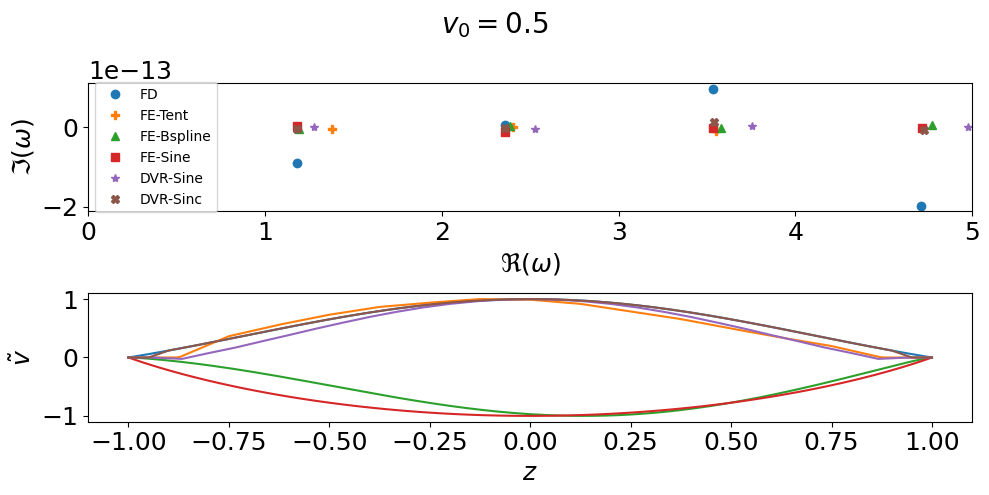
\includegraphics[width=\textwidth]{img/constant-v-Mm=0.5.png}    
            \caption{For subsonic case, the flow in magnetic nozzle is stable. The figure shows the first few modes.}
        \end{subfigure}
        \begin{subfigure}[b]{\textwidth}
            \centering
            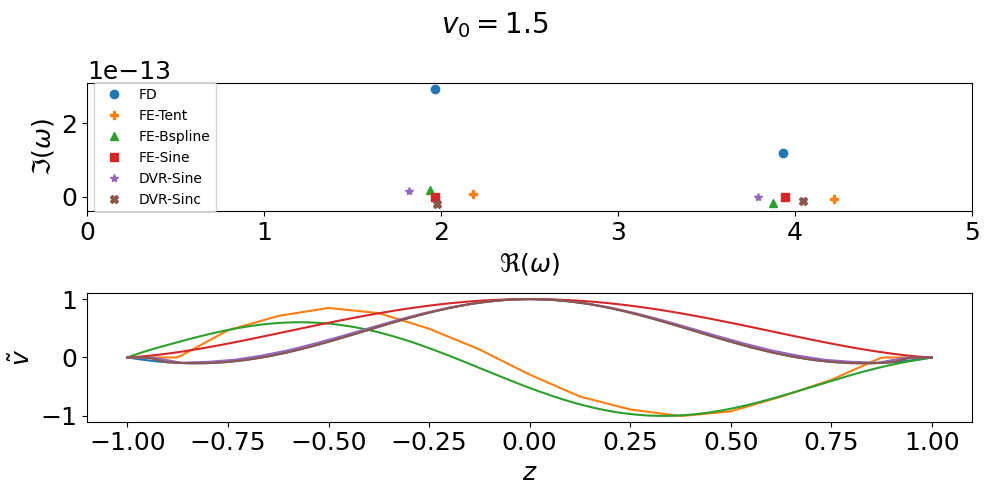
\includegraphics[width=\textwidth]{img/constant-v-Mm=1.5.png}
            \caption{For supersonic case, the flow in magnetic nozzle is also stable. The figure shows the first few modes after removing the spurious unstable modes.}
        \end{subfigure}
        \caption{The above figures show the first few modes for the flow in magnetic nozzle assuming constant velocity profile.}
    \end{figure}

    Other cases are pretty much the same. The flow in magnetic nozzle is stable.

    \bibliography{references}
    \bibliographystyle{plain}
    \nocite{smolyakov_quasineutral_2021}
\end{document}